\chapter{The Physical Basis}\label{chap:physical-basis}

\section{The Physics of Scattering}
\subsection{Radiance Attenuation}
The core physical principle behind observations performed by CPR and CALIOP is
scattering of radiation by molecules, aerosols and cloud particles. When an
electromagnetic wave passes through a particle, it can either be scattered,
absorbed, or pass unperturbed. The difference between scattering and absorption
is that in scattering, a new electromagnetic wave is generated immediately, while in
absorption, a part of the energy is absorbed, and is re-emitted later. Both
processes can be described in terms of \textit{monochromatic radiance} attenuation by the
equation:
\begin{equation}\label{eq:radiance-attenuation}
dI_\lambda = -I_\lambda \sigma_\lambda \, \mathrm{d}s
\end{equation}

\noindent where $I_\lambda$ is monochromatic radiance at wavelength $\lambda$,
$\sigma_\lambda$ is the \textit{volume extinction
coefficient} due to scattering and absorption in \SI{}{m^{-1}}, and $\mathrm{d}s$
is a
path length through the medium (air).
$\sigma_\lambda$ is a function of the medium.
Alternatively, the same can be expressed in terms of \textit{extinction
efficiency} $K_\lambda$ \citep{WallaceHobbs2006}:
\begin{equation}
dI_\lambda = -I_\lambda u N K_\lambda \, \mathrm{d}s
\end{equation}

\noindent where $N$ is the number of particles per unit volume, and $u$ is the
\textit{areal cross section} of particles\footnote{In
\cite{WallaceHobbs2006}, $u$ is denoted by $\sigma$. To avoid confusion with the
volume extinction coefficient, we changed the symbol to $u$.}.
By integrating (\ref{eq:radiance-attenuation}) from altitude $z_0$
to
$z > z_0$, we get:
\begin{equation}\label{eq:integrated-radiance-attenuation}
I_\lambda = I_{\lambda,0} e^{-\int_{z_0}^z \sigma_\lambda(z') \, \mathrm{d}z'}
\end{equation}

\noindent where $I_\lambda$ is monochromatic radiance at $z$, and $I_{\lambda,0}$ is monochromatic radiance
at $z_0$.

\noindent We define \textit{transmission} $T$ as a fraction of radiation that
passes through a slab of atmosphere:
\begin{equation}\label{eq:transmission}
T = e^{-\int_{z_0}^z \sigma(z')\,\mathrm{d}z'}
\end{equation}

\noindent (\ref{eq:integrated-radiance-attenuation}) can then be formulated as:
\begin{equation}
I_\lambda = I_{\lambda,0} T
\end{equation}

\subsection{Elastic and Inelastic Scattering}
Scattering can either be \textit{elastic} or \textit{inelastic}.
Elastic scattering occurs when there is no change in frequency of the generated
wave relative to the original wave, i.e. the particle is excited to a higher
energy state, but instantaneously returns to the original energy state.
Examples of elastic scattering are \textit{Rayleigh scattering} and \textit{Mie scattering}.
Inelastic scattering, also called \textit{Raman scattering}, the frequency of
the scattered light is either lower (\textit{Stokes scattering}) or higher
(\textit{anti-Stokes scattering}). Molecular Raman scattering can be due to
excitation of \textit{rotational} or \textit{vibrational} modes. Elastic
scattering of monochromatic light produces a so-called \textit{Cabannes line}
\citep{She2001}.

\subsection{Scattering by an Idealised Spherical Particle}
It is interesting to consider the case of an ideal spherical particle of
homogeneous material with a complex index of refraction $m = m_r + i m_i$. It
turns out that the extinction efficiency $K_\lambda$ can be expressed as a function of a
dimensionless parameter $x$ \citep{WallaceHobbs2006}:
\begin{equation}\label{eq:x}
x = 2\pi \frac{r}{\lambda}
\end{equation}

\noindent where $r$ is the radius of the particle, and $\lambda$ is the
wavelength of the incoming monochromatic plane wave.

\begin{figure}[t]
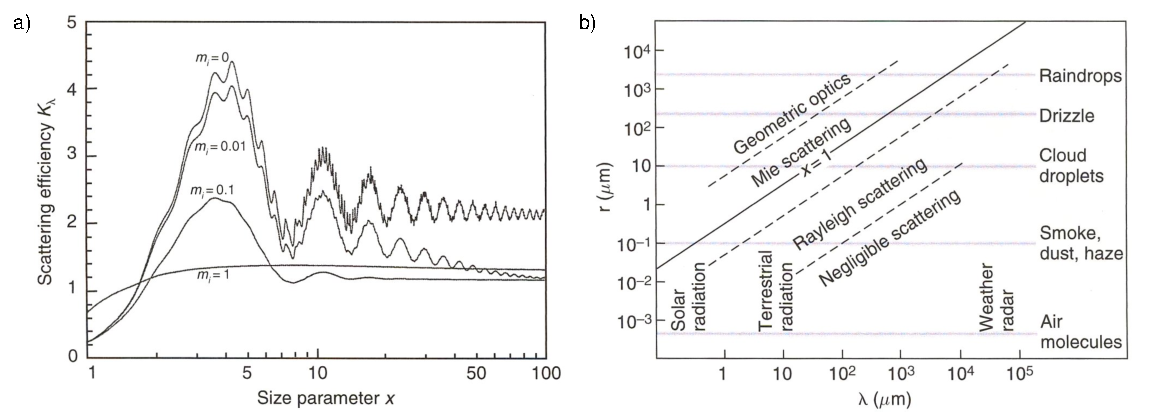
\includegraphics[width=\textwidth]{images/scattering.pdf}
\caption[Scattering by a spherical particle]{\textbf{Scattering by a spherical particle.}
\textbf{a}, Scattering efficiency $K_\lambda$ as a
function of the dimensionless size parameter $x$
for four different indices of refraction with $m_r = 1.5$.
\textbf{b}, Size parameter $x$ as a function of wavelength $\lambda$ of the
incident radiation and particle radius $r$.
[Adapted from \cite{WallaceHobbs2006}.]}
\label{fig:scattering}
\end{figure}

As you can see in Fig.\,\ref{fig:scattering}a, for $x$ approaching 1 (and in fact, for $x \leq 1$ as well), the scattering
efficiency is very low, and is proportional to $\lambda^{-4}$. This is
called the \textit{Rayleigh scattering regime}. For $0.1 \leq x \lesssim 50$,
$K_\lambda$
exhibits an oscillatory behaviour, and is referred to as the \textit{Mie
scattering regime}.
For $x \gtrsim 50$, $K_\lambda$ approaches 2. This is the \textit{geometric optics
regime}.

The parameter $x$ can give us a an impression of how strongly radiation from
CALIOP and CPR is scattered from various components of the atmosphere. For
512-nm waves, we can expect Rayleigh scattering from air molecules, Mie
scattering from aerosol particles of size \SI{10}{nm} to \SI{4}{{\textmu}m}, and
geometric reflection from water droplets and ice crystals.
For 1064-nm waves,
Rayleigh scattering from molecules should be about 16 times weaker compared to
512-nm waves (by the $\lambda^{-4}$ equation), Mie scattering can be expected
from particles of size \SI{17}{nm} to \SI{8.5}{{\textmu}m}, and geometric
reflection can be expected from cloud particles.
The situation is very different in the case of the much longer wavelength
radiation from the CPR radar. 3.2-mm waves are likely to be weakly scattered by
molecules and aerosols in the Rayleigh regime, but much more strongly scattered
from particles larger than \SI{50}{{\textmu}m}, such as cloud droplets, rain
drops, hail, and large ice crystals (Fig.\,\ref{fig:scattering}).

\section{Physics Behind CALIOP}
\subsection{The Fundamental Equation}\label{sec:caliop-the-fundamental-equation}
After a pulse of light is generated by the CALIOP laser, the receiver measures light
backscattered from molecules, aerosols and cloud particles in the atmosphere. Altitude which the
received signal relates to is inferred from delay between sending the pulse
and receiving the signal. Absorption-emission and multiple scattering are
therefore not accounted for. Moreover, the receiver subsystem contains a
narrowband filter, which only allows the Cabannes line to pass, therefore the
inelastically scattered light at different wavelengths is filtered out.
The fundamental lidar equation that relates measured signal strength $P$ to
\textit{volume backscatter coefficient} $\beta$ at range $r$ from the satellite
is \citep{PC-SCI-201}:
\begin{equation}
P(r) = E G_A C \frac{1}{r^2} \beta(r) T^2(r)
\end{equation}

\noindent where $G_A$ is the \textit{amplifier gain}, $C$ is the
\textit{calibration constant}, $E$ is the laser energy. The
$r^{-2}$ term
results from geometry of spreading out of the beam, and the coefficient $T^2$
expresses \textit{two-way attenuation} of radiation by (\ref{eq:transmission}) on
its way from the satellie at altitude $z_{sat}$ to and from the slab of air at
range $r$:
\begin{equation}
T^2(r) = e^{-2 \int\limits_{z_{sat}-r}^{z_{sat}} \sigma(z) \, \mathrm{d}z}
\end{equation}

\noindent The Level 1 products are expressed in terms of \textit{attenuated backscatter coefficient}:
\begin{equation}\label{eq:attenuated-backscatter}
\beta'(r) = \beta(r) T^2(r)
\end{equation}

\noindent Elimination of attenuation and multiple-scattering correction is the done for the Level 2 products
by the SIBYL and HERA algorithms \citep{vaughana2004}.

There are several types of backscatter coefficients. Two for the parallel and perpendicular components of the 532-nm channel ($\beta_{532,\parallel}$ and $\beta_{532,\perp}$),
one for the 1064-nm channel ($\beta_{1064}$), and the \textit{total backscatter coefficient} at \SI{532}{nm}:
\begin{equation}
\beta_{532} = \beta_{532,\parallel} + \beta_{532,\perp}
\end{equation}

\noindent All of them can be broken up into scattering due to molecules and scattering due to particulates:
\begin{equation}
\beta = \beta_m + \beta_p
\end{equation}

\noindent Attenuation is typically split into attenuation due to molecules, particulates and ozone:
\begin{equation}
T^2 = T_m^2 T_p^2 T_{O_3}^2
\end{equation}

\noindent In addition to the coefficients described above, backscatter coefficients can be combined to produce
other useful physical quantities \citep{PC-SCI-202.02}. \textit{Total color ratio} $\chi$ is defined by the equation:
\begin{equation}
\chi = \frac{\beta_{1064}}{\beta_{532}}
\end{equation}

\noindent \textit{Volume depolarization ratio} $\delta$ is defined as the ratio of the perpendicular to the parallel component of the 532-nm channel:
\begin{equation}
\delta = \frac{\beta_{532,\perp}}{\beta_{532,\parallel}}
\end{equation}

\section{Physics behind CPR}\label{sec:cpr-physics}
CPR operates by sending pulses at a wavelength of \SI{3.2}{mm}. Power received
by the antenna $P_r$ is related to the radiated power $P_t$ by the equation
\citep{1B-CPR_PDICD}:
\begin{equation}
P_r(r) = P_t \frac{1}{r^2} \frac{1}{C} \eta(r)
\end{equation}

\noindent where $r$ is the \textit{range} from the radar, $C$ is the
\textit{calibration constant}, and $\eta$ is the \textit{attenuated volume
backscatter coefficient}.
The attenuated volume backscatter coefficient
can be converted to the \textit{radar reflectivity factor} $Z$ by:
\begin{align}
\tilde{Z}^*(r) &= \frac{\lambda^4 \eta(r)}{\pi^5 |K|^2}\\
\tilde{Z}_0 &= 1 \, \mathrm{mm^6 m^{-3}}\\
Z(r) &= 10 \log_{10} \frac{\tilde{Z}^*}{\tilde{Z}_0} \, \mathrm{dBZ}
\end{align}

\noindent where $K$ is is a function of the dielectric constant (about 0.75).
The
2B-GEOPROF product contains backscatter information expressed in terms of $Z$.
Techniques of elimination of attenuation from $\eta$, and therefore retrieving
true backscatter properties at a particular range are discussed in
\cite{Li2001}.

\section{Brightness Temperature}
By treating the monochromatic radiance $I_\lambda$ as if it were emitted by a
black
body, it can be converted into so-called \textit{brightness temperature}, i.e. a
virtual
temperature of a black body emitting the same amount of radiation at a given
wavelength. It can be calculated by applying the \textit{inverse Planck function}
\citep{Houghton2002}:
\begin{equation}
T_{brightness} = \frac{c_2}{\lambda \ln\big(\frac{c_1}{\lambda^5 I_\lambda} +
1\big)}
\end{equation}

\noindent where $c_1$ and $c_2$ are the \textit{first} and \textit{second
radiation constants}:
\begin{align}
c_1 &= 1.1911 \times 10^{-8} \, \mathrm{W m^{-2} sr^{-1}
\left(cm^{-1}\right)^{-4}}\\
c_2 &= 1.439 \, \mathrm{K \left(cm^{-1}\right)^{-1}}
\end{align}

\noindent Brightness temperature can be used when visualising MODIS thermal
emission bands instead of monochromatic radiance.
